\title{Nonparametric Goodness-of-Fit Tests for Discrete Null Distributions}
\author{by Taylor B. Arnold and John W. Emerson}

\maketitle

\abstract{
Methodology extending nonparametric goodness-of-fit tests
to discrete null distributions has existed
for several decades. However, modern statistical software
has generally failed to provide this methodology
to users. We offer a revision of R's \code{ks.test()} function
and a new \code{cvm.test()} function that fill this need
in the R language for two of the most popular nonparametric
goodness-of-fit tests. This paper describes these contributions and
provides examples of their usage. Particular attention is given
to various numerical issues that arise in their implementation.
}



\section{Introduction}

%General idea of goodness-of-fit tests (hypothesis test about underlying distribution).
%Given an observed sequence of data, the typical question of statistical inference is to determine
%the underlying process from which it came. 
Goodness-of-fit tests are used to assess whether data are consistent
with a hypothesized null distribution.  The $\chi^2$ test is the best-known
parametric goodness-of-fit test, while the most popular nonparametric tests
are the classic test proposed by Kolmogorov and Smirnov followed closely by
several variants on Cram\'{e}r-von Mises tests.

%procedure proposed by
%Cram\'{e}r and von Mises (tests sometimes called Cram\'{e}r-von Mises-Smirnov
%tests, or simply Cram\'{e}r-von Mises tests).

%*** why "estimation procedure" above?
%*** Citations in the paragraph above?  Also check the body of paper. ***

In their most basic forms, these nonparametric goodness-of-fit
tests are intended for continuous null distributions, but they have
also been adapted for discrete null distributions.  Unfortunately,
most modern statistical software packages and programming environments
have failed to incorporate these discrete versions.  As a result,
researchers would typically rely upon the $\chi^2$ test or
use of a nonparametric test designed for a continuous null distribution.
For smaller sample sizes, in particular, both of these choices can produce
misleading inferences.

This paper presents a revision of R's
\code{ks.test()} function and a new \code{cvm.test()} function to
fill this void for researchers and practitioners in the R environment. 
We first present overviews of the theory and general implementation of the
discrete Kolmogorov-Smirnov and Cram\'{e}r-von Mises tests.  We discuss
the particular implementation of tests in R and provide examples.  We
conclude with a short discussion, including the state of existing continuous
and two-sample Cram\'{e}r-von Mises testing in R.

%*** Later, make sure we point out how using one of the ``old'' tests and
%hoping for the best is a problem. ***

%Given a particular null distribution, goodness-of-fit tests 
%are used in order to test whether it is likely that the data were
%generated via the null distribution.

%Why we use non-parametric tests (power to interesting shifts; robustness to underlying assumptions).
%While almost any hypothesis test can be viewed as a variant on a
%goodness-of-fit test, the term ``goodness-of-fit test'' is typically
%reserved for those tests which are nonparametric in nature. 
%That is, they do not conduct the hypothesis testing 
%through the explicit calculation of the parameters generating the data. Instead, they %generally attempt to
%calculate differences between the empirical distribution of the observed data and the overall distribution 
%of the null model. In many cases these tests are preferential since they tend to have an increased power for 
%interesting deviations from the null model, in exchange for failing to detect less interesting deviations due to 
%factors such as measurement error. By far the most popular of these nonparametric tests are due to Kolmogorov and 
%Smirnov, followed closely by several variants on an estimation procedure proposed by Cram\'{e}r and von Mises. 

% Discrete versions exist; just no code
%While the original aim of nonparametric goodness of fit tests was meant for continuous null distributions, discrete versions
%have existed since the early 1970s. Unfortunately, current statistical software has largely failed to incorporate them.
%This has left the end-user to either use only parametric tests, such as Pearson's Chi-Squared test, or to incorrectly
%apply the functions meant for continuous distributions. 

\section{Kolmogorov-Smirnov Test}

% Most popular choice of test; explain the basic algorithm and purpose for continuous distributions (maybe a few P's).

\subsection{Overview}

The most popular nonparametric goodness-of-fit test is the
Kolmogorov-Smirnov test.
Given the cumulative distribution
function $F_0(x)$ of the continuous null distribution
and the empirical distribution function $F_{data}(x)$ of the observed data,  the test statistic is given by
\begin{align}
D = \sup_x \left| F_0(x)- F_{data}(x) \right|.    \label{eqD}
\end{align}
The distribution of $D$ does not depend on the hypothesized
distribution, making this a computationally
attractive method. \cite{slakter65} offers a standard presentation
of the test and its
performance relative to other algorithms. 
The test statistic is easily adapted for one-sided tests.
For these, the absolute value in (\ref{eqD}) is discarded and the tests are based
on either the supremum of the remaining difference (the `greater' testing
alternative) or by replacing the supremum with a negative infimum
(the `lesser' hypothesis alternative).  Tabulated p-values have been
available for these tests since 1933. %(*** year ****).

%**** check this above, both do away with the absolute value, I think? ***

The extension of the Kolmogorov-Smirnov test to non-continuous 
null distributions is not straightforward. The formula of
the test statistic $D$ remains unchanged, but its distribution
is much more difficult to obtain; unlike the 
continuous case, its distribution depends on the null model.
It has been known since at least the 1950's that using the tables associated
with continuous null distributions results in conservative p-values
when the null distribution is discontinuous 
(see *** or *** or \citet{stephens1974}, for example).  In the early 1970's, 
\citet{Conover1972} developed the method implemented here
for computing exact p-values
in the case of discrete null distributions.

\subsection{Implementation}

The implementation of the discrete Kolmogorov-Smirnov test involves
two steps. First, the particular test statistic is calculated
(corresponding to the desired one-sided or two-sided test).
Then, the p-value for that particular test statistic may be computed. 

The form of the test statistic is the same as in the
continuous case; it would seem that no additional work would be required
for the implemenetation, but this is not the case.
Consider two non-decreasing functions $f$ and $g$, where the function $f$ is a step function with jumps on the set $\{x_1, \ldots x_N \}$ and $g$
is continuous (the classical Kolmogorov-Smirnov situation).
In order to determine the supremum of the difference between
these two functions, notice that **** FORMAT THESE AT END ****
\begin{align}
&\sup_x \left| f(x)- g(x) \right|  \nonumber  \\
       &= \max_i \left( \max\left\{ \left|g(x_i) - f(x_i) \right|, \lim_{x \rightarrow x_i} \left| g(x) - f(x_{i-1}) \right| \right\} \right) \label{SUP1}\\
&=  \max_i \bigg(\max \bigg\{ \left|g(x_i) - f(x_i) \right|, \left| g(x_i) - f(x_{i-1}) \right| \bigg\} \bigg). \label{SUP2}
\end{align}
Computing the maximum over these $2N$
values (with $f$ equal to
$F_{data}(x)$ and $g$ equal to $F_0(x)$ as defined above) is clearly the 
most efficient way to compute the Kolmogorov-Smirnov test statistic for
a continuous null distribution. When the function $g$ is not
continuous, however, equality (\ref{SUP2}) does not hold in general because 
we cannot replace $\lim_{x\rightarrow x_i} g(x)$ with the value $g(x_i)$. 

If it is known that $g$ is a step function, it follows that
for some small $\epsilon$,
\begin{align}
\sup_x &\left| f(x)- g(x) \right| =  \nonumber \\
        &                    \max_i \{ \left|g(x_i) - f(x_i) \right|, \left| g(x_i - \epsilon) - f(x_{i-1}) \right| \} \label{epsilon}
\end{align}
where the discontinuities in $g$ are more than some distance $\epsilon$ apart. 
This, however, requires knowledge that $g$ is a step function as well as of
the nature of its support (or break-points).
%
%*** Hmm... do we care about time? ***  When the break-points of $g$ are
%unknown, or when $g$ is neither a step function nor a continuous distribution
%function, computing the supremum requires taking the numerical limit in (1***?). 
%This is computational involved and risks problems with numerical tolerances.
%
We implement the Kolmogorov-Smirnov test statistic for discrete null
distributions by forcing the user to completely specify the null distribution.

%**** Hmmm... It is often the case that the test is used inside of a
%long simulation, 
%and the added computational time would likely be prohibitive. 

Having obtained the test statistic, the p-value must then be calculated. 
For larger sample sizes, the null distribution can be approximated
with the null distribution from the classical Kolmogorov-Smirnov test. 
When an exact p-value is required for
smaller sample sizes, the methodology in \citet{Conover1972} is used. 
Full details of the calculations are contained in source code
of our revised function \code{ks.test()} and in Conover's original paper. 

%** code hasn't previously existed?  I deleted this stuff, not sure if
%it fits here.  Is it obvious (since we bothered to do this in the first
%place)?  Or move it?

%Code for this procedure in the R language, or in any other open source options, did not previously
%exist and is included in the new function \pkg{ks.test}. 

%Numerical issues arise from the summation; need to do something else for high $n$. Simulation? Asymptotic approximation? 
%The interesting part of the implementation of Conover's method, from a computational standpoint, are the difficult numerical issues that 
%arise when calculated the p-values for larger sample sizes. 

\section{Cram\'{e}r-von Mises Tests}

\subsection{Overview}

%General idea for continuous distributions. In many cases actually more powerful of the two. There again exists a distribution free 
%distribution for the testing statistic.

While the Kolmogorov-Smirnov test may be the most popular of
the nonparametric goodness-of-fit tests, there is another family of 
tests which has been shown to be more powerful against a large class
of alternatives hypotheses. 
The original test was developed by
Harald Cram\'{e}r and Richard von Mises \citep{cramer1928, vonmises1928} and further adapted by \cite{anderson1952}, and  \cite{Watson1961}. 
The original test statistic, $W^2$, Anderson's $A^2$, and Watson's
$U^2$ are:
\begin{align}
W^2 &= n \cdot \int_{-\infty}^{\infty} \left[ F_{data}(x)- F_{0}(x) \right]^2 dF_0(x) \label{W2} \\
A^2 &= n \cdot \int_{-\infty}^{\infty} \frac{\left[F_{data}(x)- F_{0}(x) \right]^2}{F_0(x) -F_0(x)^2} dF_0(x) \label{A2} \\
U^2 &= n \cdot \int_{-\infty}^{\infty} \left[ F_{data}(x)- F_{0}(x) - W^2 \right]^2 dF_0(x) \label{U2}
\end{align}
As with the original Kolmogorov-Smirnov test statistic, these all have 
null distributions of their test statistics which are independent of the
specified null models.

The $W^2$
statistic was the original test statistic; it has the benefit of having
the simplest form.
The $A^2$ statistic was developed by
Anderson in the process of generalizing the test for the two-sample case.
Watson's $U^2$ statistic was developed for distributions
which are cyclic (with an ordering to the support but
no natural starting point), as it is invariant to cyclic reordering of
the support. 
For example, a distribution on the months of the year could be considered
cyclic.

It has been shown that these tests can be more powerful than Kolmogorov-Smirnov tests to certain deviations from the hypothesized distribution. 
As they all involve
integration over the whole range of data, rather than use of a supremum.
Thus, they are best-suited for situations where the
true alternative distribution deviates a little over the whole support
rather than having large deviations over a small section of the support. For
a complete analysis of the relative powers of these tests, see 
\cite{stephens1974}.

%Discuss the discrete version. How to calculate W2, U2, and A2. 

%*** I edited, below, make sure you check it. ****

Generalizations of the Cram\'{e}r-von Mises tests to discrete
distributions were developed in \cite{choulakian1994}. As with the
Kolmogorov-Smirnov test, the forms of the test statistics are unchanged, 
and the null distributions of the test statistics are again hypothesis-dependent. The methods do not offer finite-sample results, but rather 
show that the asymptotic distributions of the test statistics under the null hypothesis each involve consideration of a weighted sum of independent
chi-squared variables (with the weights depending on the particular
null distribution). 
We implement the asymptotic distributions here; \cite{stephens1974}
showed that these approximations are conservative 
and asymptotically equivalent to the true null distributions.


\subsection{Implementation}

Calculation of the three test statistics is done using the
matrix algebra given by \cite{choulakian1994}. 
The only notable difficulty in the implementation of the discrete form
of the tests involves calculating the percentiles
of the weighted sum of chi-squares,
\begin{align}
Q = \sum_{i=1}^{p} \lambda_i \chi^2_{i,1df},   \label{eqQ}
\end{align}
where $p$ is the number of elements in the support of the hypothesized
distribution.
\cite{imhof1961} provides a method for obtaining the distribution of $Q$,
easily adapted for our case because
the chi-squared variables have only one degree of freedom.
The exact formula given for the distribution function of $Q$
is given by
\begin{align}
\mathbb{P}\{Q \geq x \} = \frac{1}{2} + 
\frac{1}{\pi} \int_{0}^{\infty} \frac{\sin\theta(u,x)}{u \rho(u) } du
\label{distQ}
\end{align}
for continuous functions $\theta(\cdot, x)$ and $\rho(\cdot)$ depending on the  weights $\lambda_i$. 

There is no analytic solution to the integral in (\ref{distQ}), 
so the integration is
accomplished numerically. This seems fine in most situations we considered,
but numerical issues appear in the regime of large test statistics $x$
(or, equivalently, small p-values).
The function $\theta(\cdot, x)$ is linear in $x$; as the test statistic 
grows the corresponding periodicity of the integrand decreases and
the approximation becomes unstable. 
%This is further magnified in situations where the 
%$p$-values should be very small, where tiny fluctuations (undetectable
%elsewhere) become quite prominent. 
We resolve this problem by using a simple conservative approximation to
avoid the numerical instability. Consider the
following inequality:
\begin{align}
\mathbb{P} \left(\sum_{i=1}^{p} \lambda_i \chi^2_1 \geq x \right) &\leq \mathbb{P} \left( \lambda_{max} \sum_{i=1}^{p} \chi^2_1 \geq x \right) \label{ineq1} \\
&= \mathbb{P} \left(\chi^2_p \geq \frac{x}{p \, \lambda_{max}} \right)
\label{ineq2}
\end{align}
The values for the weighted sum can be bounded using a simple transformation
and a chi-squared distribution of a higher degree of freedom. 
The original formulation is preferable for most p-values, while
this approximation is used for smaller p-values (smaller than 0.001,
based on our observations of the numerical instability of the original
formulation).

Figure \ref{cvmissues} shows the non-monotonicity of the numerical
evaluation of equation (\ref{distQ}) for the null distribution which is
uniform on the set $\{1,2,3\}$, as well as the behavior of the
conservative upper bound given in equation (\ref{ineq2}).

\begin{figure}
\begin{center}
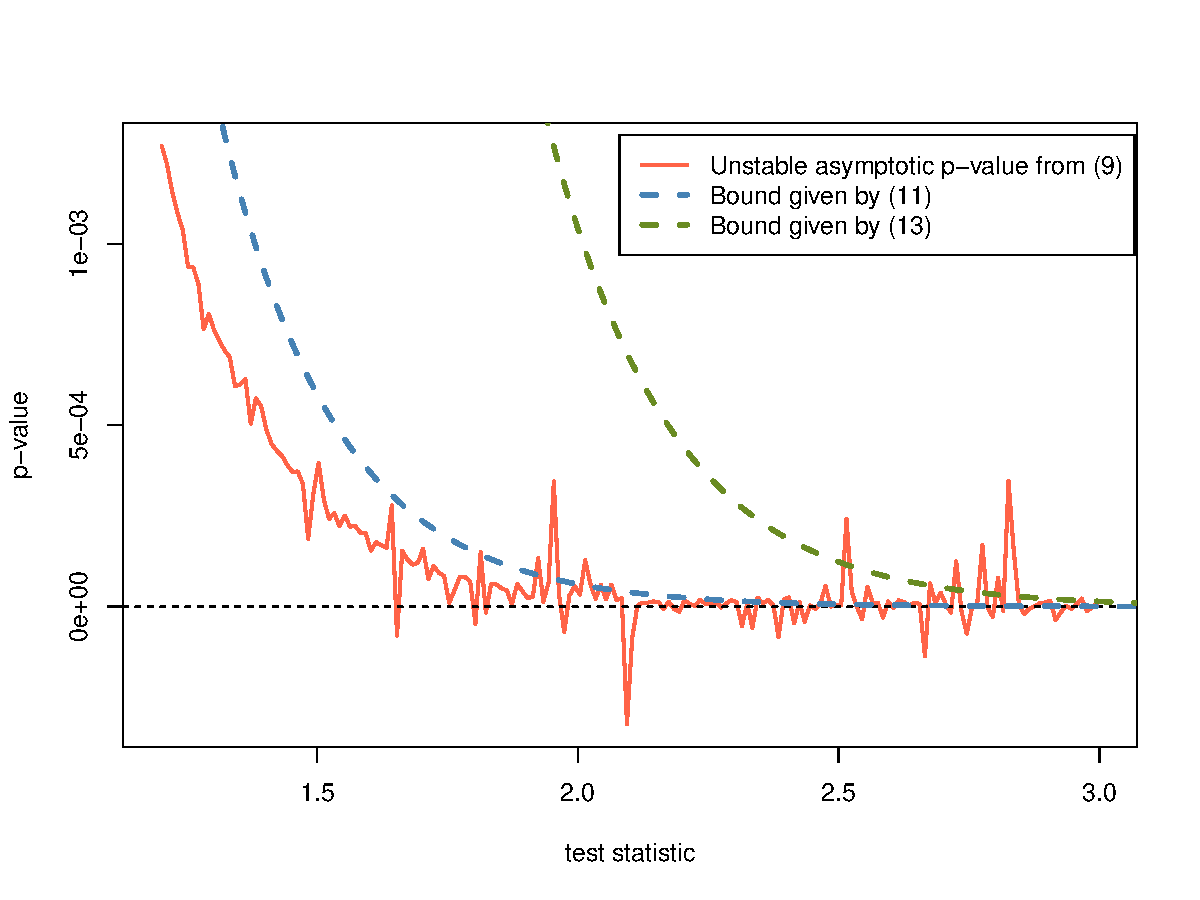
\includegraphics[scale=0.4]{fig1.pdf}
\end{center}
\caption{Plot of calculated p-values for given test statistics
using numerical integration
(pink) compared to the conservative chi-squared bound (dashed blue). 
The null distribution is uniform on the set $\{1,2,3\}$ in this example.
The instability in the calculated p-values is a result of numerical
instabilities.}
\label{cvmissues}
\end{figure}


%%%%%%%%%%%%%%%%%%%%%%%%%%%%%%%%%%%%%%%%%%%%%%%%%%%%%%
\section{Kolmogorov-Smirnov and Cram\'{e}r-von Mises Tests in R}

Functions \code{ks.test()} and \code{cvm.test()} are provided for
convenience in packages \pkg{ks.test} and \pkg{cvm.test}, respectively.
Function \code{ks.test()} offers a revision of
R's Kolmogorov-Smirnov function \code{ks.test()} from base
package \pkg{stats}, while \code{cvm.test()} is a new
function for Cram\'{e}r-von Mises tests.
Both are available from the authors
or from R-Forge (\url{https://r-forge.r-project.org/R/?group_id=802});
they will be proposed for inclusion in \pkg{stats} in late 2010.

The revised \code{ks.test()} function supports one-sample tests for discrete
null distributions by allowing the second argument, \code{y}, to be
an empirical cumulative distribution function (an R function
with class \code{ecdf}) or an object of class \code{stepfun} specifying
a discrete distribution.  As in the original version of \code{ks.test()},
the presence of ties in the data (the first argument, \code{x}) generates a
warning unless \code{y} describes a discrete distribution.  When a discrete
distribution is specified, exact p-values are not available for 
two-sided alternative hypotheses, but the reported p-values will be
conservative.  For one-sided tests,
exact p-values are calculated using Conover's
method (when \code{exact = NULL} or \code{exact = TRUE})
if the sample size is less than or equal to 30; otherwise, asymptotic distributions
are used which are reliable in such cases (CITATION? Is this correct?).
When \code{exact = FALSE} the asymptotic distribution is used which is known
to be imprecise but conservative, even for small samples (CITATION).

%*** Discussion of what we might have broken: cases where the user
%provided a discrete distribution to the original ks.test() even though
%it wasn't intended to be supported. ***

The function \pkg{cvm.test()} is similar to \pkg{ks.test()}.  Its first two
arguments specify the data and null distribution; the only extra option,
\code{type}, specifies the variant of the Cram\'{e}r-von Mises test:
\begin{itemize}
\item \code{x}: a numerical vector of data values.
\item \code{y}: an \code{ecdf} or step-function (\code{stepfun}) for specifying
the null model
\item \code{type}: the variant of the Cram\'{e}r-von Mises test; \code{W2}
is the default and most common method, \code{U2} is for cyclical data,
and \code{A2} is the Anderson-Darling alternative.
\end{itemize}
As with \code{ks.test()}, \code{cvm.test()} returns an object of class 
\code{htest}.

 
%%%%%%%%%%%%%%%%%%
\section{Examples}

Consider a toy example, with observed data of length 2 (specifically, the
values 0 and 1) and a hypothized null distribution that places equal
probability on the values 0 and 1.  With the current \code{ks.test()} function
in R (which, admittedly, doesn't claim to handle discrete distributions),
the reported p-value, 0.5, is clearly incorrect:
\begin{Schunk}
\begin{Sinput}
> stats::ks.test(c(0, 1), ecdf(c(0, 1)))
\end{Sinput}
\begin{Soutput}
	One-sample Kolmogorov-Smirnov test

data:  c(0, 1) 
D = 0.5, p-value = 0.5
alternative hypothesis: two-sided 
\end{Soutput}
\end{Schunk}
Instead, the value of $D$ given in equation (1)
should be 0 and the associated p-value should be 1.  Our revision of \code{ks.test()}
fixes this problem when the user provides a discrete distribution:
\begin{Schunk} 
\begin{Sinput}
> ks.test(c(0, 1), ecdf(c(0, 1)))
\end{Sinput}
\begin{Soutput}
	One-sample Kolmogorov-Smirnov test

data:  c(0, 1) 
D = 0, p-value = 1
alternative hypothesis: two-sided 
\end{Soutput}
\end{Schunk}

Next, we simulate a sample of 25 from the discrete uniform distribution on
the integers $\{1, 2, \ldots, 10\}$ and show several variants of the
new \code{ks.test()} implementation.  The first is the default two-sided test,
where the reported p-value is a conservative upper bound for the actual
p-value.  In this case, the approximation may not be that tight, but this is
irrelevant for such large p-values (for more interesting p-values, the
upper bound is very close to the true p-value).
\begin{Schunk}
\begin{Sinput}
> library(ks.test)
> set.seed(1)
> x <- sample(1:10, 25, replace = TRUE)
> x
\end{Sinput}
\begin{Soutput}
 [1]  3  4  6 10  3  9 10  7  7  1  3  2  7
[14]  4  8  5  8 10  4  8 10  3  7  2  3
\end{Soutput}
\begin{Sinput}
> ks.test(x, ecdf(1:10))
\end{Sinput}
\begin{Soutput}
	One-sample Kolmogorov-Smirnov test

data:  x 
D = 0.08, p-value = 1
alternative hypothesis: two-sided 
\end{Soutput}
\end{Schunk}
Next, we conduct the default one-sided test, where Conover's method
provides the exact p-value (up to the numerical precision of the
implementation):
\begin{Schunk}
\begin{Sinput}
> ks.test(x, ecdf(1:10), alternative = "g")
\end{Sinput}
\begin{Soutput}
	One-sample Kolmogorov-Smirnov test

data:  x 
D^+ = 0.04, p-value = 0.7731
alternative hypothesis:
the CDF of x lies above the null hypothesis 
\end{Soutput}
\end{Schunk}
In contrast, the option \code{exact=FALSE} results in the
p-value obtained by applying the classical Kolmogorov-Smirnov
test, resulting in a conservative p-value:
\begin{Schunk}
\begin{Sinput}
> ks.test(x, ecdf(1:10), alternative = "g", 
+         exact = FALSE)
\end{Sinput}
\begin{Soutput}
	One-sample Kolmogorov-Smirnov test

data:  x 
D^+ = 0.04, p-value = 0.9231
alternative hypothesis:
the CDF of x lies above the null hypothesis 
\end{Soutput}
\end{Schunk}
A different toy example shows the dangers of using R's existing
\code{ks.test()} function:
\begin{Schunk}
\begin{Sinput}
> ks.test(rep(1, 3), ecdf(1:3))
\end{Sinput}
\begin{Soutput}
	One-sample Kolmogorov-Smirnov test

data:  rep(1, 3) 
D = 0.6667, p-value = 0.04938
alternative hypothesis: two-sided 
\end{Soutput}
\end{Schunk}
If, instead, either \code{exact=FALSE} is used with the new
\code{ks.test()} function, or if the original \code{stats::ks.test()}
is used, the reported p-value is 0.1389.

Finally, we employ two of the Cram\'{e}r-von Mises tests.  Need short discussion,
and we could use a good cyclical example:
\begin{Schunk}
\begin{Sinput}
> library(cvm.test)
> cvm.test(x, ecdf(1:10))
\end{Sinput}
\begin{Soutput}
	Cramer-von Mises - W2

data:  x 
W2 = 0.057, p-value = 0.8114
alternative hypothesis: Two.sided 
\end{Soutput}
\begin{Sinput}
> cvm.test(x, ecdf(1:10), type = "A2")
\end{Sinput}
\begin{Soutput}
	Cramer-von Mises - A2

data:  x 
A2 = 0.3969, p-value = 0.75
alternative hypothesis: Two.sided 
\end{Soutput}
\end{Schunk}

Cyclical example:

\begin{Schunk}
\begin{Sinput}
> library(cvm.test)
> x <- sample(1:4, 20, replace=T)
> cvm.test(x, ecdf(1:4), type='U2')
\end{Sinput}
\begin{Soutput}
	Cramer-von Mises - U2

data:  x 
U2 = 0.075, p-value = 0.4027
alternative hypothesis: Two.sided 
\end{Soutput}
\begin{Sinput}
> y <- x%%4 + 1
> cvm.test(y, ecdf(1:4), type = 'U2')
\end{Sinput}
\begin{Soutput}
	Cramer-von Mises - U2

data:  y 
U2 = 0.075, p-value = 0.4027
alternative hypothesis: Two.sided 
\end{Soutput}
\end{Schunk}




\section{Discussion}

%*** I commented out a bunch of stuff.  I think the discussion can be short
%and sweet. ***

%The chi-squared test is a popular alternative to the methods presented here for doing goodness-of-fit tests for discrete data.
%It differs by using no information about the geometry of the distribution, instead relying only the difference between the 
%number of data points observed at each value and the expected number of data points that should be observed at each point. 
%This generally has the effect of having a greater power towards alternatives with sharply different densities on a few points,
%at the expense of losing power for alternatives with slight deviations over all of the points. Also, the non-parametric tests
%have an advantage of being useful when the sample size is lower compared to the support of the distribution. The chi-squared
%test is generally not used unless there are at least five data points in each element of the support. On the other hand,
%chi-squared can be used in situations when there is not a numerical interpretation of the observation space 
%(e.g. a set of ethnicities).
%For a more complete comparison of the two tests' power see \cite{slakter65}.

%The computational capabilities of modern computers provide an alternative to using a complex formula to
%calculate the p-value for a test statistic. By drawing random samples from the null distribution, in many
%cases the p-values for a given statistic can be calculated accurately in a relatively short time span.
%This can be quite useful in some cases, but using the exact formulas from our methodology has several
%distinct advantages. First of all, if the function is called many times (say, within another simulation
%study), the computational benefits of using a formula can quickly become substantial. There is also a greater need
%for supervision in a simulation study, with the exact number of runs needed to reach convergence (or other 
%similar threshold). Additionally, while
%simulations are generally a well received accepted method, it is often important in applied data analysis
%to be sure that the calculated $p$-values are not the result of a numerical oddity in a particular
%run of a simulation. 

%*** Hmm... if you claim the following, you want to make sure it is true.
%Did you read it somewhere? ***

In the end, for methods such as those presented in this paper where it is possible,
there are enough positives to suggest that we attempt to implement exact $p$-value calculations. This does lead
to an interesting direction for future research in non-parametric goodness of fit tests: the methods presented
here were historically chosen because they could be shown to have fixed null distributions which could easily
calculated in an era without fast computers for carrying out permutation tests. It is quite possible that
variants without the property, which could be easily used today, have greater power to certain alternative 
distributions.

%Possibly go into a brief discussion of classes and class inheritance in R. The use of `htest' in our functions; benefits and issues with using it. Particularly troublesome in ks.test where we have a range of p-values.  More precisely, explain that we
%could provide upper and lower bounds for the p-value but are limited by class
%\code{htest}.

In the continuous setting, both of 
the Kolmogorov-Smirnov and the Cram\'{e}r-von Mises tests have two-sample analogues. Here data are
observed from two processes, and the hypothesis tested is 
whether they came from the same (but unspecified) distribution. There
does not exist an analogous theory for discrete distributions. 
This comes from the fact that the discrete null distributions
of the test statistics depend on the exact null distribution; 
therefore the two-sample case would surely have to depend
on the exact distributions used as well %(*** is this true? ***), 
which are generally not even stated in the two-sample case. 

While we have implemented the two most popular variants of 
goodness-of-fit tests, there are 
several more exotic varieties to be found. For further 
generalizations of tests see the extended study done in \cite{dewev1973}.


%\bibliography{example}

\bibliography{paper}

\address{Taylor B. Arnold \\
Yale University\\
24 Hillhouse Ave. \\
New Haven, CT 06511
USA\\
}
\email{taylor.arnold@yale.edu}

\address{John W. Emerson \\
Yale University\\
24 Hillhouse Ave. \\
New Haven, CT 06511
USA\\
}
\email{john.emerson@yale.edu}

